\chapter{Roleplays}

\section*{What are roleplays?}
\begin{quote}
A roleplay is a 10-minute presentation to a volunteer judge with 10 minutes of preparation. 
In those 10 minutes of your presentation, you be graded on your ability to explain the Performance Indicators 
in a comprehensive and creative way. Additionally, you will also be graded on 21st century skills
which all total up to a composite maximum score of 100 points per roleplay. 
\end{quote} 

\section*{How are they graded}
\begin{quote}
You will be given approximately 5 PI's and the 5 base 21st Century Skills.
Totaling up, you can obtain a max score of 100. Attached below is an example
rubric from a practice roleplay.

\end{quote}

\begin{figure}[H]
    \center
    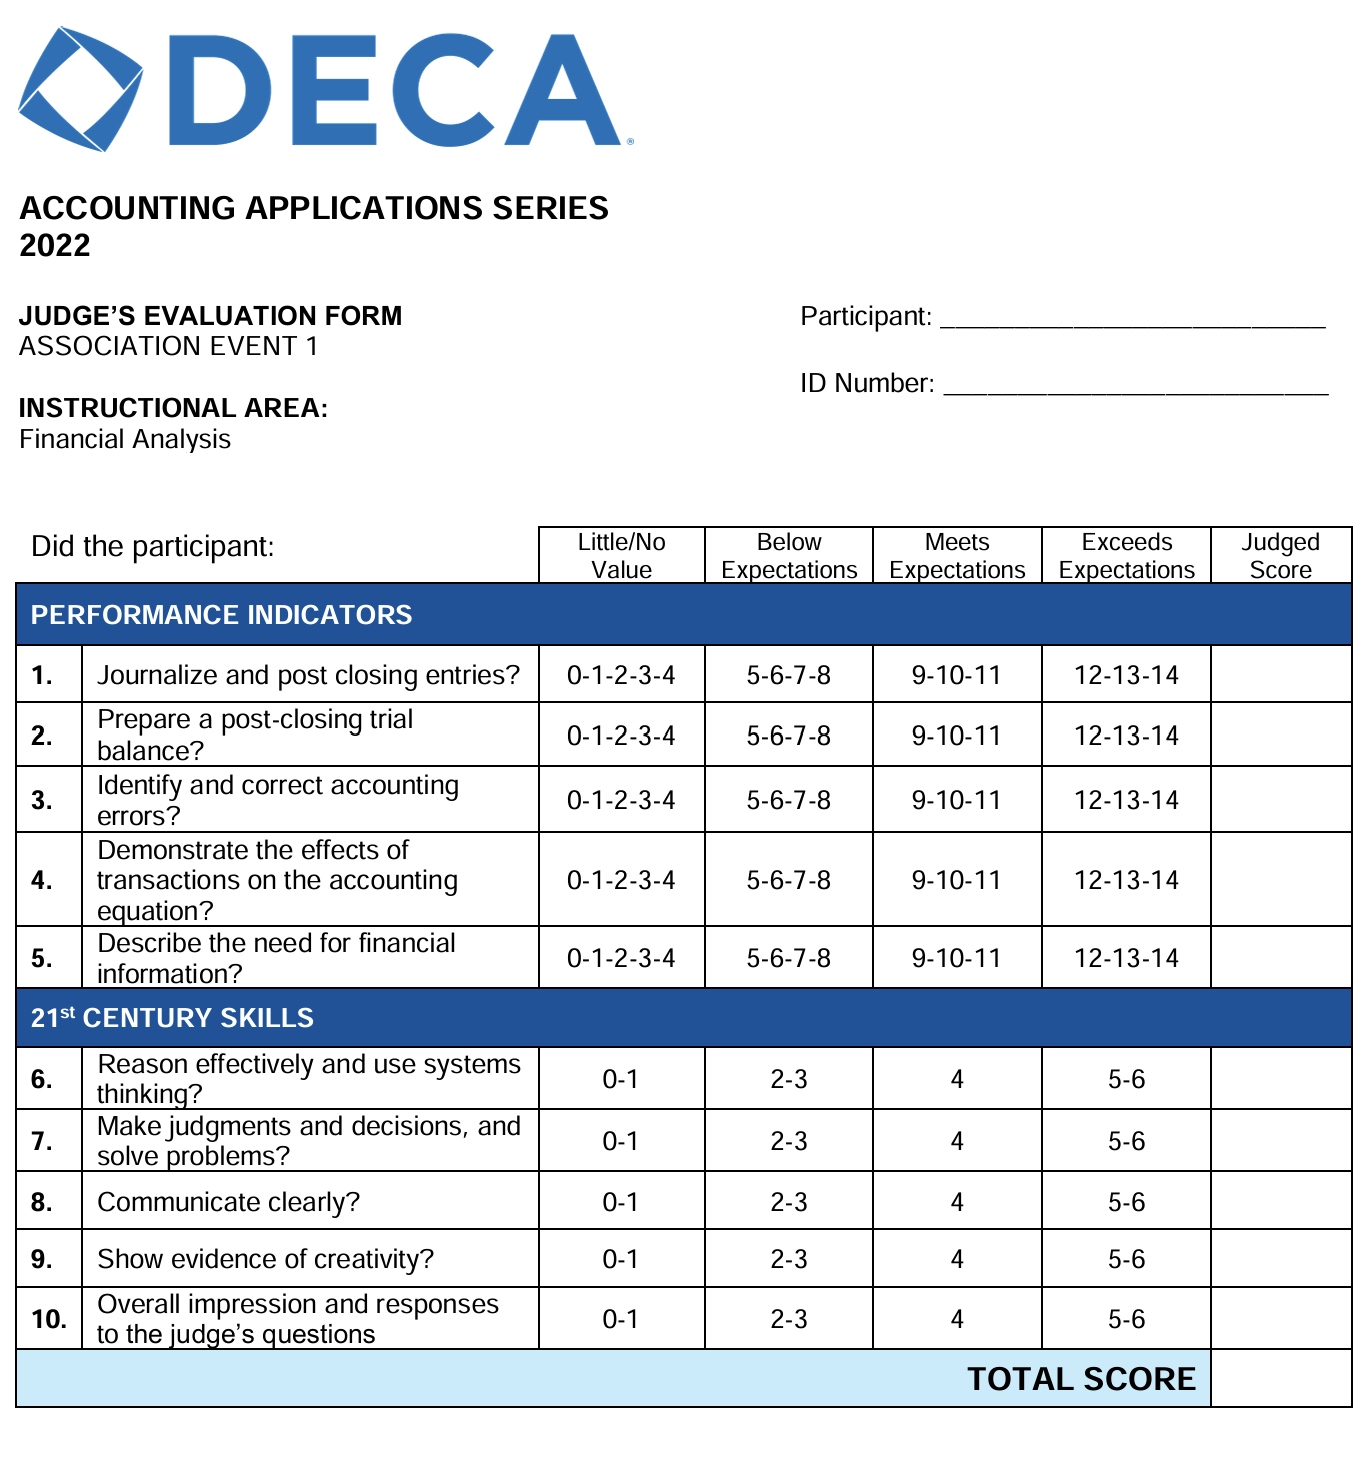
\includegraphics[width=1\textwidth,height=1\textheight,keepaspectratio]{grading.png}
    \caption[short]{ACT-22 Practice Roleplay Rubric}
\end{figure}

\section*{How to do a Roleplay}

\subsection*{Preparation}
\begin{enumerate}
    \item Read PI's 
    \item Plan how you would describe them in a way that is related to the roleplay.
    \item Focus on PI's and also a solution to the roleplay that incoporates those PI's
    \item Create Visuals: Large Topic, 3-4 Bullet Points, Picture/Graph 
    \item ACT Visuals include: Financial Statements, Journal Entries, etc.
    \item Visual example
    \begin{figure}[H]
        insert visual example 
    \end{figure}
    \item REPEAT until done 
\end{enumerate}

\subsection*{Presenting | Structure}
\begin{enumerate}
    \item Introduction
        \begin{itemize}
            \item Name
            \item Company
            \item Background
            \item Permission to sit down
        \end{itemize}
    \item Agenda
        \begin{itemize}
            \item Before we get started here is a breakdown of what I'll be showing today
            \item List PI's
        \end{itemize}
    \item Explaning
        \begin{itemize}
            \item Begin explaining \key{ALL PI's} using the DECA acronym
            \item \key{D:} Describe
            \item \key{E:} Explain
            \item \key{C:} Connect
            \item \key{A:} Actions
        \end{itemize}
    \item Recap (Agenda p2)
        \begin{itemize}
            \item Summarize everything you discussed about
            \item Clarify and Solidify any topics
            \item Talk about CTA (Call to Action)
            \item \key{Ask for questions!}
        \end{itemize}
    \item Questions \key{[CALM DOWN]}
        \begin{itemize}
            \item Usually 2 Questions
            \item Make or Breaks.
            \item You can bs this. 
        \end{itemize}
\end{enumerate}


\section*{KEY Tips}

\begin{itemize}
    \item THEY ARE VOLUNTEERS, Always assume they aren't real accountants so \key{explain very thoroughly}.
    \item Always connect the PI's back to the roleplay.
    \item Make sure to always \key{SMILE}
    \item Eye Contact is key.
    \item Confidence is king.
    \item Fake it until you make it.
    \item Leave 1-2 minutes for questions
    \item Write the company name \& position behind your agenda.
\end{itemize}